\subsection{可测等价关系}

给定一个拓扑空间 X 与 X 中的一个等价关系 R ，若商空间 X/R 是 Hausdorff 空间，我们就说 R 是 Hausdorff 的。

回忆（GT, I, §8, No.~3, 命题 8），当 R 是一个开等价关系时，说 R 在 X × X 中的图是闭的，这与说 R 是开的等价。

设 p 是 X 到一个 Hausdorff 拓扑空间 B 中的映射， R 是 X 中由 \(p(x) = p(y)\) 定义的等价关系；若 K 是 X 的一个紧子集，使得 p 在 K 上的限制连续，则 R 在 K 上诱导的等价关系 \(R_{K}\) 是 Hausdorff 的，因为商空间 \(K/R_{K}\) 同胚于空间 \(p(K)\) ，后者是紧的（GT, I, §9, No.~4, 定理 2 及其推论 2）。若 T 是局部紧空间， \(\mu\) 是 T 上的正测度， p 是 T 到一个 Hausdorff 拓扑空间 B 中的 \(\mu\) -可测映射，那么由此看出，存在 T 的紧子集的一个 \(\mu\) -稠密族（Ch. IV, §5, No.~8），对其中的 K ，关系 \(R_{K}\) 是 Hausdorff 的。这样我们就被引导到下述定义：

定义 3. --- 设 T 是局部紧空间， \(\mu\) 是 T 上的正测度。 T 中的等价关系 R 称为 \(\mu\) -可测的，如果存在 T 的紧子集的一个 \(\mu\) -稠密族，对其中的 K ，关系 \(R_{K}\) 是 Hausdorff 的。

若 R 是 Hausdorff 的，则 R 是 \(\mu\) -可测的，因为若 \(\varphi\) 是 T 到 Hausdorff 拓扑空间 T/R 上的典范映射，则 \(\varphi\) 连续且 R 等价于 \(\varphi(x)=\varphi(y)\) 。类似地，若 R 使得 T 的每个紧子集关于 R 的饱和集是闭的（特别地，若 R 是闭等价关系），则 R 是 \(\mu\) -可测的，因为对 T 的每个紧子集 K ，关系 \(R_{K}\) 是闭的，从而是 Hausdorff 的（GT, I, §10, No.~4, 命题 8）。

注意，若 R 是 \(\mu\) -可测的，则 R 对 T 上每个以 \(\mu\) 为基的测度也是可测的。

命题 2. --- 设 T 是一个无穷远处可数的局部紧空间， \(\mu\) 是 T 上的正测度。

\begin{enumerate}
\def\labelenumi{\arabic{enumi})}
\item
  对 T 中每个 \(\mu\) -可测等价关系 R ，存在一个局部紧空间 B 和 T 到 B 中的一个 \(\mu\) -可测映射 p ，使得 R 等价于关系 \(p(x) = p(y)\) 。
\item
  此外，若 T 具有可数基，则可以假定 B 也具有可数基。
\end{enumerate}

由于 T 无穷远处可数，存在 T 的紧子集的一个递增序列 \((\mathrm{K}_{n})_{n\geqslant1}\) ，使得 T 是诸 \(K_{n}\) 与一个 \(\mu\) -可忽略集 N 的并，且使得诸关系 \(R_{K_{n}}\) 中的每一个都是 Hausdorff 的。设 \(B_{n}\) 是商空间 \(K_{n}/R_{K_{n}}\) ，它是紧的，又设 \(B_{n}^{\prime}\) 是由 \(B_{n}\) 与一点 \(a_{n}\) 的拓扑和所成的紧空间。设 \(q_{n}\) 是 \(K_{n}\) 到 \(B_{n}\) 上的典范映射；我们按如下方式把 \(q_{n}\) 延拓为一个映射 \(p_{n}\) （ T 到 \(B_{n}^{\prime}\) 中的映射）：若 \(x\in T\) 模 R 等价于一个元素 \(y\in K_{n}\) ，令 \(p_{n}(x)=q_{n}(y)\) ；相反的情形，令 \(p_{n}(x)=a_{n}\) 。设 \(B^{\prime}\) 是乘积空间 \(\prod_{i=1}^{\infty}B_{n}^{\prime}\) ，它是紧的，又设 \(p^{\prime}\) 是 T 到 B' 中的映射 \(x \mapsto (p_n(x))\) 。我们来证明 \(p'\) 是 \(\mu\) -可测的：只需（Ch. IV, §5, No.~3, 定理 1）证明每个映射 \(p_n\) 可测，而为此只需 \(p_n\) 在每个 \(K_m\) 上的限制可测。现在，若 \(m \leqslant n\) ，这是显然的；相反，若 m \textgreater{} n ，设 \(K_{nm}\) 是 \(K_n\) 关于 \(R_{K_m}\) 的饱和集，它是 \(K_m\) 的一个紧子集（GT, I, §9, No.~4, 定理 2）；由于 \(p_n\) 在 \(K_m - K_{nm}\) 上是常数，只需证明 \(p_n\) 在 \(K_{nm}\) 上的限制连续，而这由 \(K_{nm}/R_{K_{nm}}\) 与 \(K_n/R_{K_n}\) 之间的典范同构看出（GT, I, §9, No.~4, 定理 2 的推论 4）。

设 A 是 \(\bigcup_{n} \mathrm{K}_{n}\) 关于关系 R 的饱和集，并设 \(\mathrm{N}' = \mathrm{T} - \mathrm{A} \subset \mathrm{N}\) 。我们将看到，关系 \(p'(x) = p'(y)\) 等价于关系 \(\langle \mathrm{R}\{x, y\}\) 或 \((x, y) \in \mathrm{N}' \times \mathrm{N}' \rangle\) 。因为，若 \(\mathrm{R}\{x, y\}\) ，则 \(p_n(x) = p_n(y)\) （对一切 \(n\) ），从而 \(p'(x) = p'(y)\) ；又若 \(x \in \mathrm{N}'\) ， \(y \in \mathrm{N}'\) ，则 \(p_n(x) = p_n(y) = a_n\) （对一切 \(n\) ），从而 \(p'(x) = p'(y)\) 。另一方面，若 \(x\) 与 \(y\) 都属于 A 且不模 R 等价，则存在一个整数 \(n\) 、一个元素 \(x' \in \mathrm{K}_n\) （相应地， \(y' \in \mathrm{K}_n\) ）模 R 等价于 \(x\) （相应地， \(y\) ），使得 \(x'\) 不等价于 \(y'\) （模 \(\mathrm{R}_{\mathrm{K}_n}\) ）；因此 \(p_n(x) \neq p_n(y)\) ，从而 \(p'(x) \neq p'(y)\) 。最后，若 \(x \in \mathrm{N}'\) 且 \(y \in \mathrm{A}\) ，则 \(p_n(y) \in \mathrm{B}_n\) （对充分大的 \(n\) ），且 \(p_n(x) = a_n\) （对一切 \(n\) ），因此 \(p'(x) \neq p'(y)\) ，这就证明了我们的断言。

于是考虑商集 \(B_{0} = N^{\prime}/R_{N^{\prime}}\) ；设 \(q_{0}\) 是 \(N^{\prime}\) 到 \(B_{0}\) 上的典范映射， \(s_{0}\) 是 \(q_{0}\) 的一个截面。令 \(p_{0}(x) = s_{0}(q_{0}(x))\) （对 \(x \in N^{\prime}\) ），并把 \(p_{0}\) 延拓到 T 上，办法是取 \(p_{0}\) 在 A 上等于 T 中一个元素（常值）。于是 \(p = (p^{\prime}, p_{0})\) 是一个 \(\mu\) -可测映射（ T 到局部紧空间 \(B = B^{\prime} \times T\) 中的映射）；直接看出，若 \(x \in N^{\prime}\) ， \(y \in N^{\prime}\) ，则关系 \(p_{0}(x) = p_{0}(y)\) 蕴含 \(R\{x, y\}\) ；因而 p 满足所要求的条件。此外，若 T 具有可数基，则每个商空间 \(B_{n}\) 也具有可数基（GT, IX, §2, No.~10, 命题 17），因此 \(B^{\prime}\) 具有可数基，从而 B 也具有可数基。

命题 3. --- 设 T 是一个 Polish 局部紧空间， \(\mu\) 是 T 上的正测度， R 是 T 中的一个等价关系。下列性质等价：

\begin{enumerate}
\def\labelenumi{\alph{enumi})}
\item
  R 是 \(\mu\) -可测的。
\item
  存在取值于 Hausdorff 拓扑空间的映射的一个序列 \(p_n: \mathrm{T} \to \mathrm{F}_n\) ，使得每个 \(p_n\) 是 \(\mu\) -可测的，且使得关系 \(\mathrm{R}\{x, y\}\) 等价于«对一切 \(n\) ， \(p_n(x) = p_n(y)\) »。
\item
  存在一个序列 \((\mathrm{A}_{n})\) （ \(\mu\) -可测集的序列），它们关于 R 是饱和的，使得对每个 \(x \in T\) ， x 关于 R 的类是包含 x 的那些 \(A_{n}\) 的交。
\end{enumerate}

采用叙述 \(b\) 中的记号，令 \(p(x) = (p_n(x))\) ；性质 \(b\) 意味着映射 \(p\) （ \(T\) 到乘积空间 \(\prod_{n} F_n\) 中的映射）可测（Ch. IV, §5, No.~3, 定理 1），且关系 \(R\{x, y\}\) 等价于 \(p(x) = p(y)\) ；于是 \(b\) ）蕴含 \(a\) 。

其次我们证明 \(c)\) 蕴含 \(b)\) 。设 \(c)\) 成立；则特征函数 \(\varphi_{\mathrm{A}_n}\) 是 \(\mu\) -可测的，且假设 \(c)\) 意味着关系 \(\mathrm{R}\{x, y\}\) 等价于«对每个 \(n\) ， \(\varphi_{\mathrm{A}_n}(x) = \varphi_{\mathrm{A}_n}(y)\) »。

最后我们证明 \(a)\) 蕴含 \(c)\) 。由命题 2，存在一个具有可数基的局部紧空间 B 和 T 到 B 中的一个 \(\mu\) -可测映射 \(p\) ，使得关系 \(\mathrm{R}\{x,y\}\) 等价于 \(p(x)=p(y)\) 。设 \((\mathrm{U}_{n})\) 是 B 的拓扑的一个可数基。诸集 \(\mathrm{A}_{n}=\overline{p}^{-1}(\mathrm{U}_{n})\) 是 \(\mu\) -可测的（Ch. IV, §5, No.~5, 命题 7）且关于 R 饱和；且若 \(x,y\) 是 T 中使 \(p(x)\neq p(y)\) 的点，则存在一个指标 \(n\) ，使得 \(p(x)\in\mathrm{U}_{n}\) 而 \(p(y)\notin\mathrm{U}_{n}\) ，这就意味着 \(x\in\mathrm{A}_{n}\) 而 \(y\notin\mathrm{A}_{n}\) 。

\pandocbounded{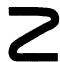
\includegraphics[keepaspectratio]{images/part003_0d7fd957.jpg}}

注记. --- 若 R 是 T 中的一个 \(\mu\) -可测等价关系， T 的紧子集关于 R 的饱和集未必是 \(\mu\) -可测的（习题 5）。

定理 3. --- 设 T 是一个具有可数基的局部紧空间， \(\mu\) 是 T 上的正测度， R 是 T 中的一个 \(\mu\) -可测等价关系。则存在 T 的一个 \(\mu\) -可测子集 S ，它与每个关于 R 的类恰好交于一点（ R 的一个「可测截面」）。

我们显然可以假定测度 \(\mu\) 有界且 \(\mu(T) \leqslant 1\) （Ch. V, §5, No.~6, 命题 11）。我们将定义 Borel 子集的一个序列 \((S_n)\) （GT, IX, §6, No.~3），使得每个关于 R 的等价类与并 \(S'\) （诸 \(S_n\) 之并）至多交于一点，使得对每个 \(n\) ，饱和集 \(T_n\) （诸 \(S_p\) （指标 \(p \leqslant n\) ）的并的饱和集）是 \(\mu\) -可测的，且使得 \(\mu(T - T_n) \leqslant 1/2^n\) 。于是饱和集 \(T'\) （ \(S'\) 的饱和集）将是 \(\mu\) -可测的，而 \(N = T - T'\) 将具有零测度。若 \(S''\) 是 N 关于关系 \(R_N\) 的任意一个截面，则 \(S = S' \cup S''\) 就满足所要求的条件，因为 \(S'\) 是 Borel 集，故 \(\mu\) -可测（Ch. IV, §5, No.~4, 定理 2 的推论 3），而 \(S''\) 具有零测度。

由命题 2， \(\mathrm{R}\{x,y\}\) 等价于关系 \(p(x)=p(y)\) ，其中 \(p\) 是 T 到一个局部紧空间 F 中的 \(\mu\) -可测映射。设 \(\mathrm{S}_{k}\) 已对 \(k\leqslant n\) 定义。由于 \(\mathrm{T}-\mathrm{T}_{n}\) 是 \(\mu\) -可测的且测度 \(\leqslant 1/2^{n}\) ，存在 \(\mathrm{T}-\mathrm{T}_{n}\) 的一个紧子集 K ，使得 \(\mu\big(\mathrm{T}-(\mathrm{T}_{n}\cup\mathrm{K})\big)\leqslant 1/2^{n+1}\) 且 \(p\) 在 K 上的限制连续。由于诱导的关系 \(\mathrm{R}_{\mathrm{K}}\) 是闭的且 K 可度量化，我们知道存在 K 的一个 Borel 子集 \(\mathrm{S}_{n+1}\) ，使得在 K 中每个点都（模 R ）等价于 \(\mathrm{S}_{n+1}\) 中恰好一点（GT, IX, §6, No.~8, 定理 4）。因此 \(p(\mathrm{S}_{n+1})=p(\mathrm{K})\) ，它是 F 中的紧集； \(\mathrm{S}_{n+1}\) 关于 R 的饱和集是逆像 \(\overline{p}^{-1}(p(\mathrm{K}))\) ，因而它是 \(\mu\) -可测的（Ch. IV, §5, No.~5, 命题 7）；显然这个集包含 K ，因此并 \(\mathrm{T}_{n+1}\) （ \(\mathrm{T}_n\) 与 \(\overline{p}^{-1}(p(\mathrm{K}))\) 的并）是 \(\mu\) -可测的、关于 R 饱和的，且使得 \(\mu(\mathrm{T} - \mathrm{T}_{n+1}) \leqslant 1/2^{n+1}\) ，证明至此完成。

